\documentclass{beamer}
\usepackage[orientation=portrait, size=a1]{beamerposter}

\usepackage{polyglossia}
\setmainfont{Liberation Serif}
\setsansfont{Liberation Sans}
\setmonofont{Liberation Mono}

\begin{document}
\centering
\Huge
\hfill
\\
\vspace{2em}
Алгоритм функционирования метода выявления скрытых процессов
\vfill
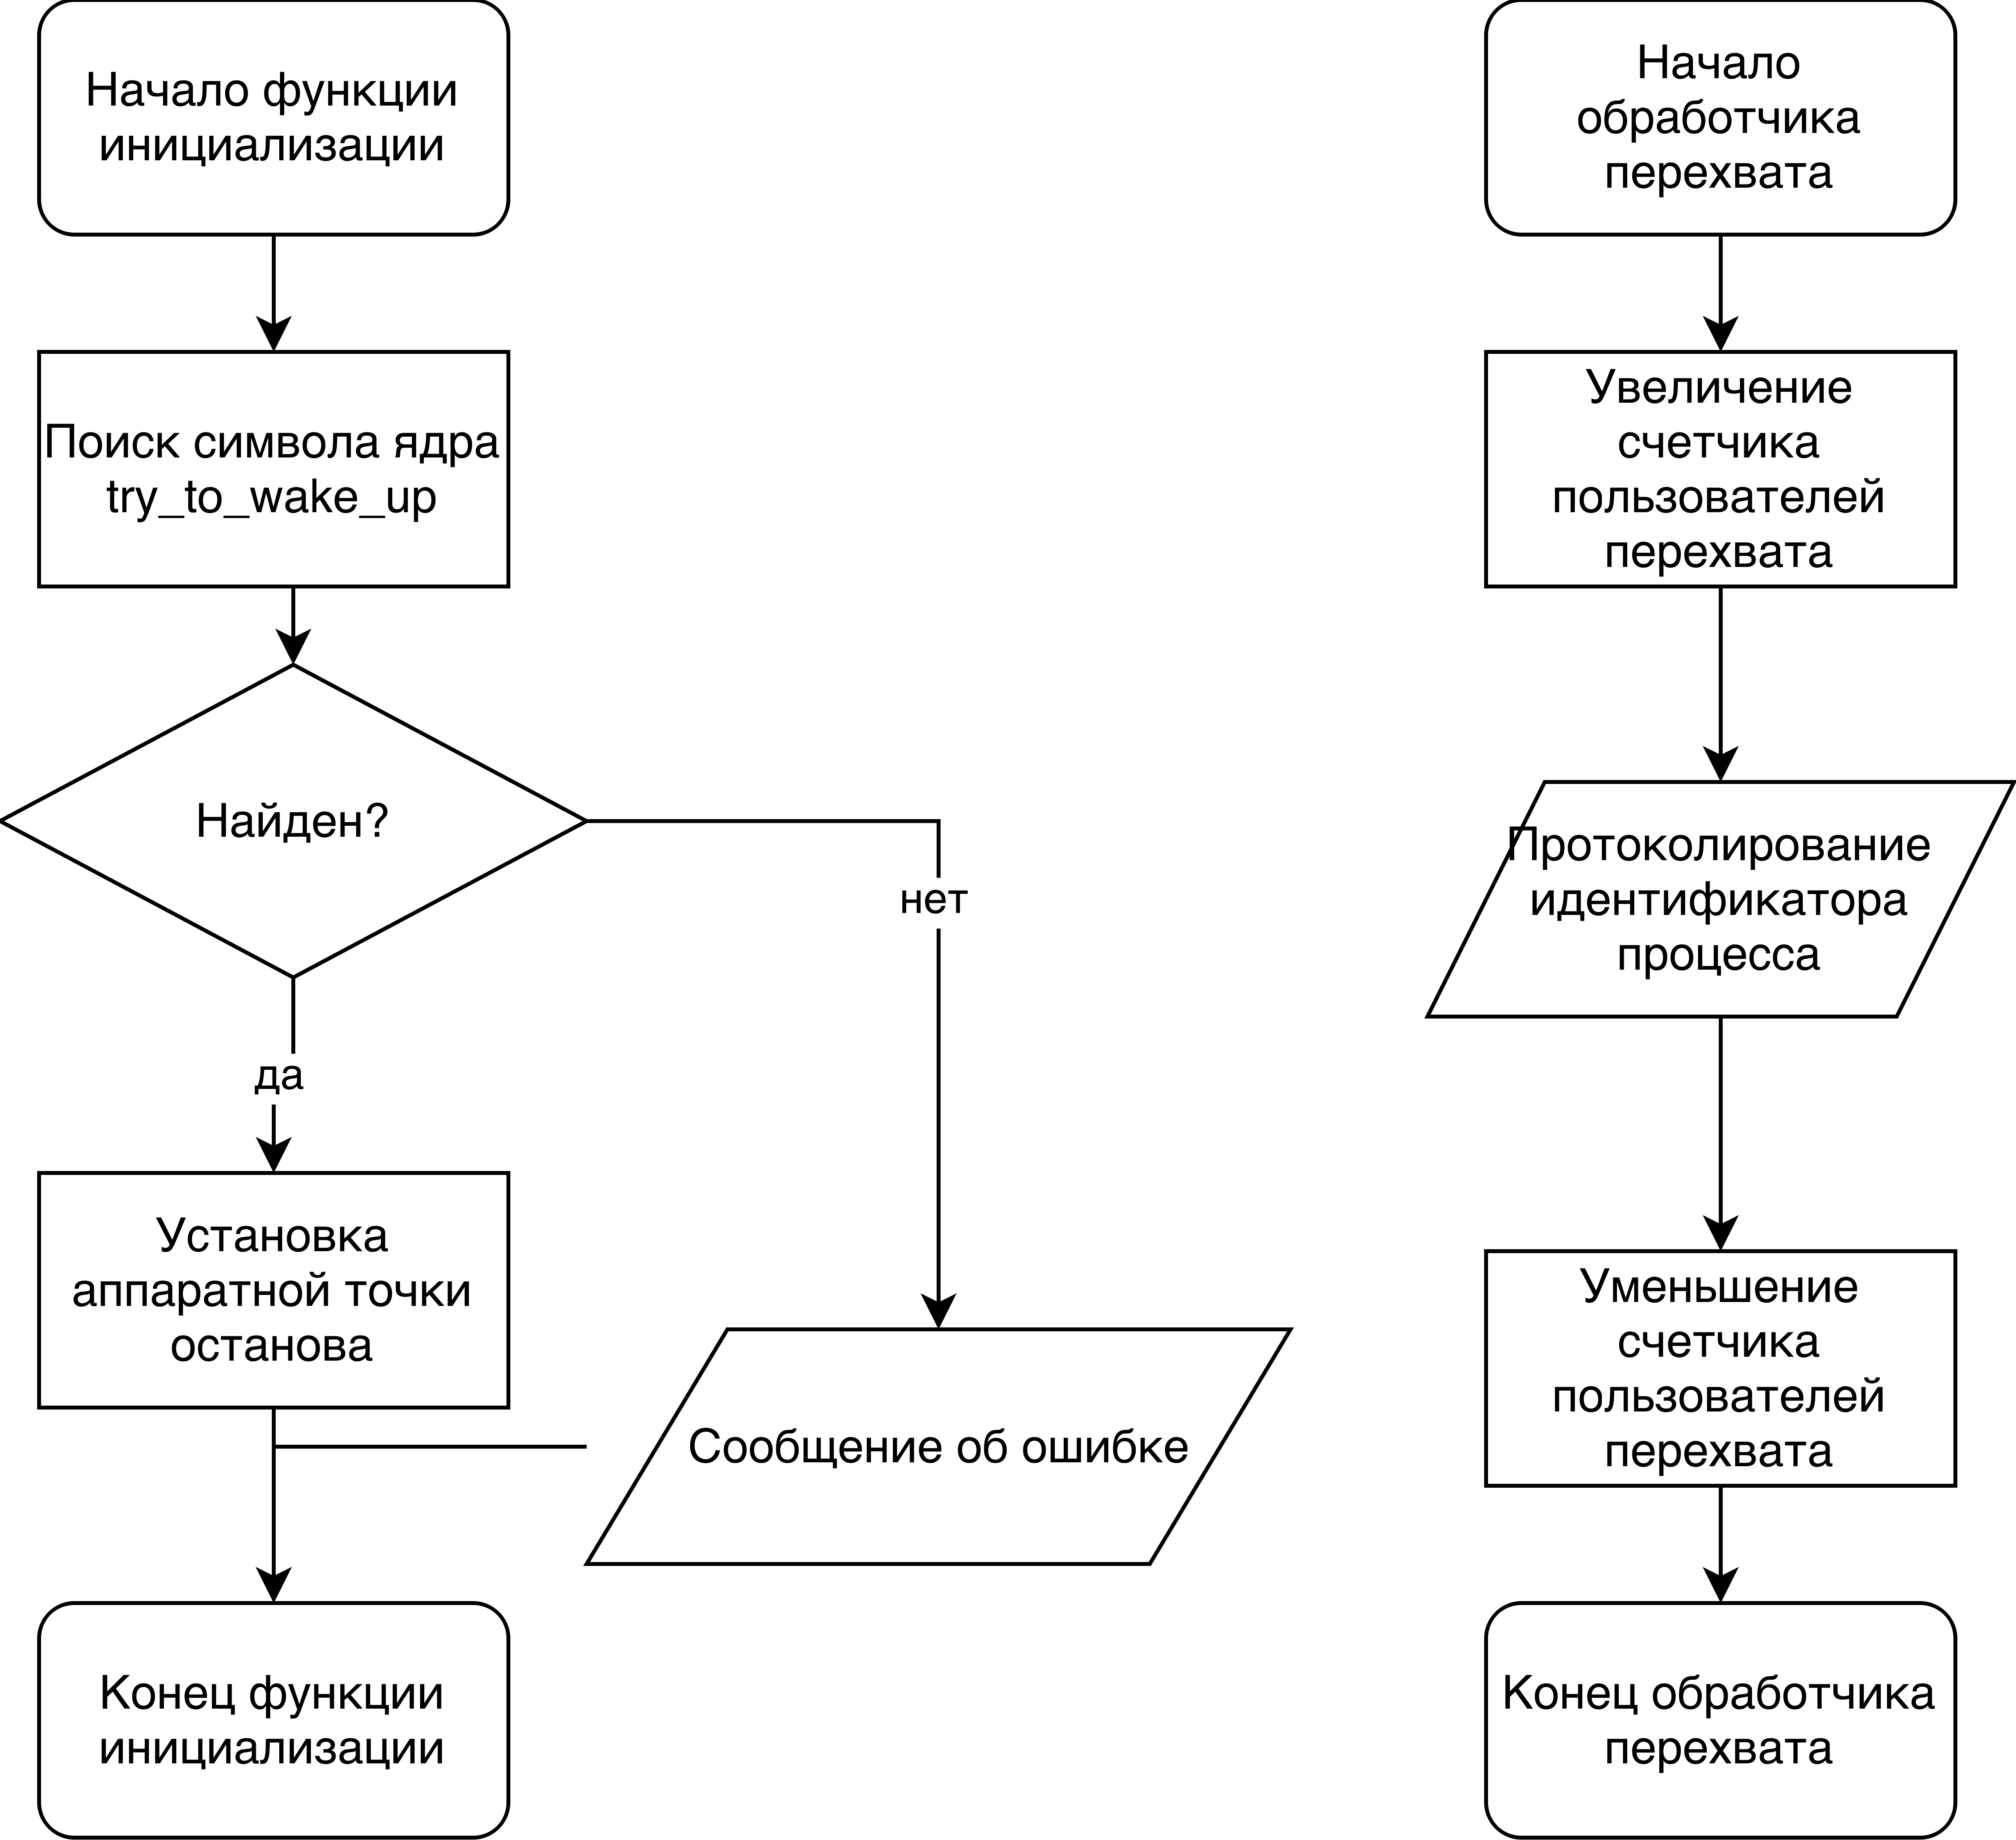
\includegraphics[width=0.9\textwidth]{images_posters/hook_scheduler.png}
\vfill

\newpage
\hfill
\\
\vspace{2em}
Алгоритм функционирования метода выявления скрытых сетевых соединений
\vfill
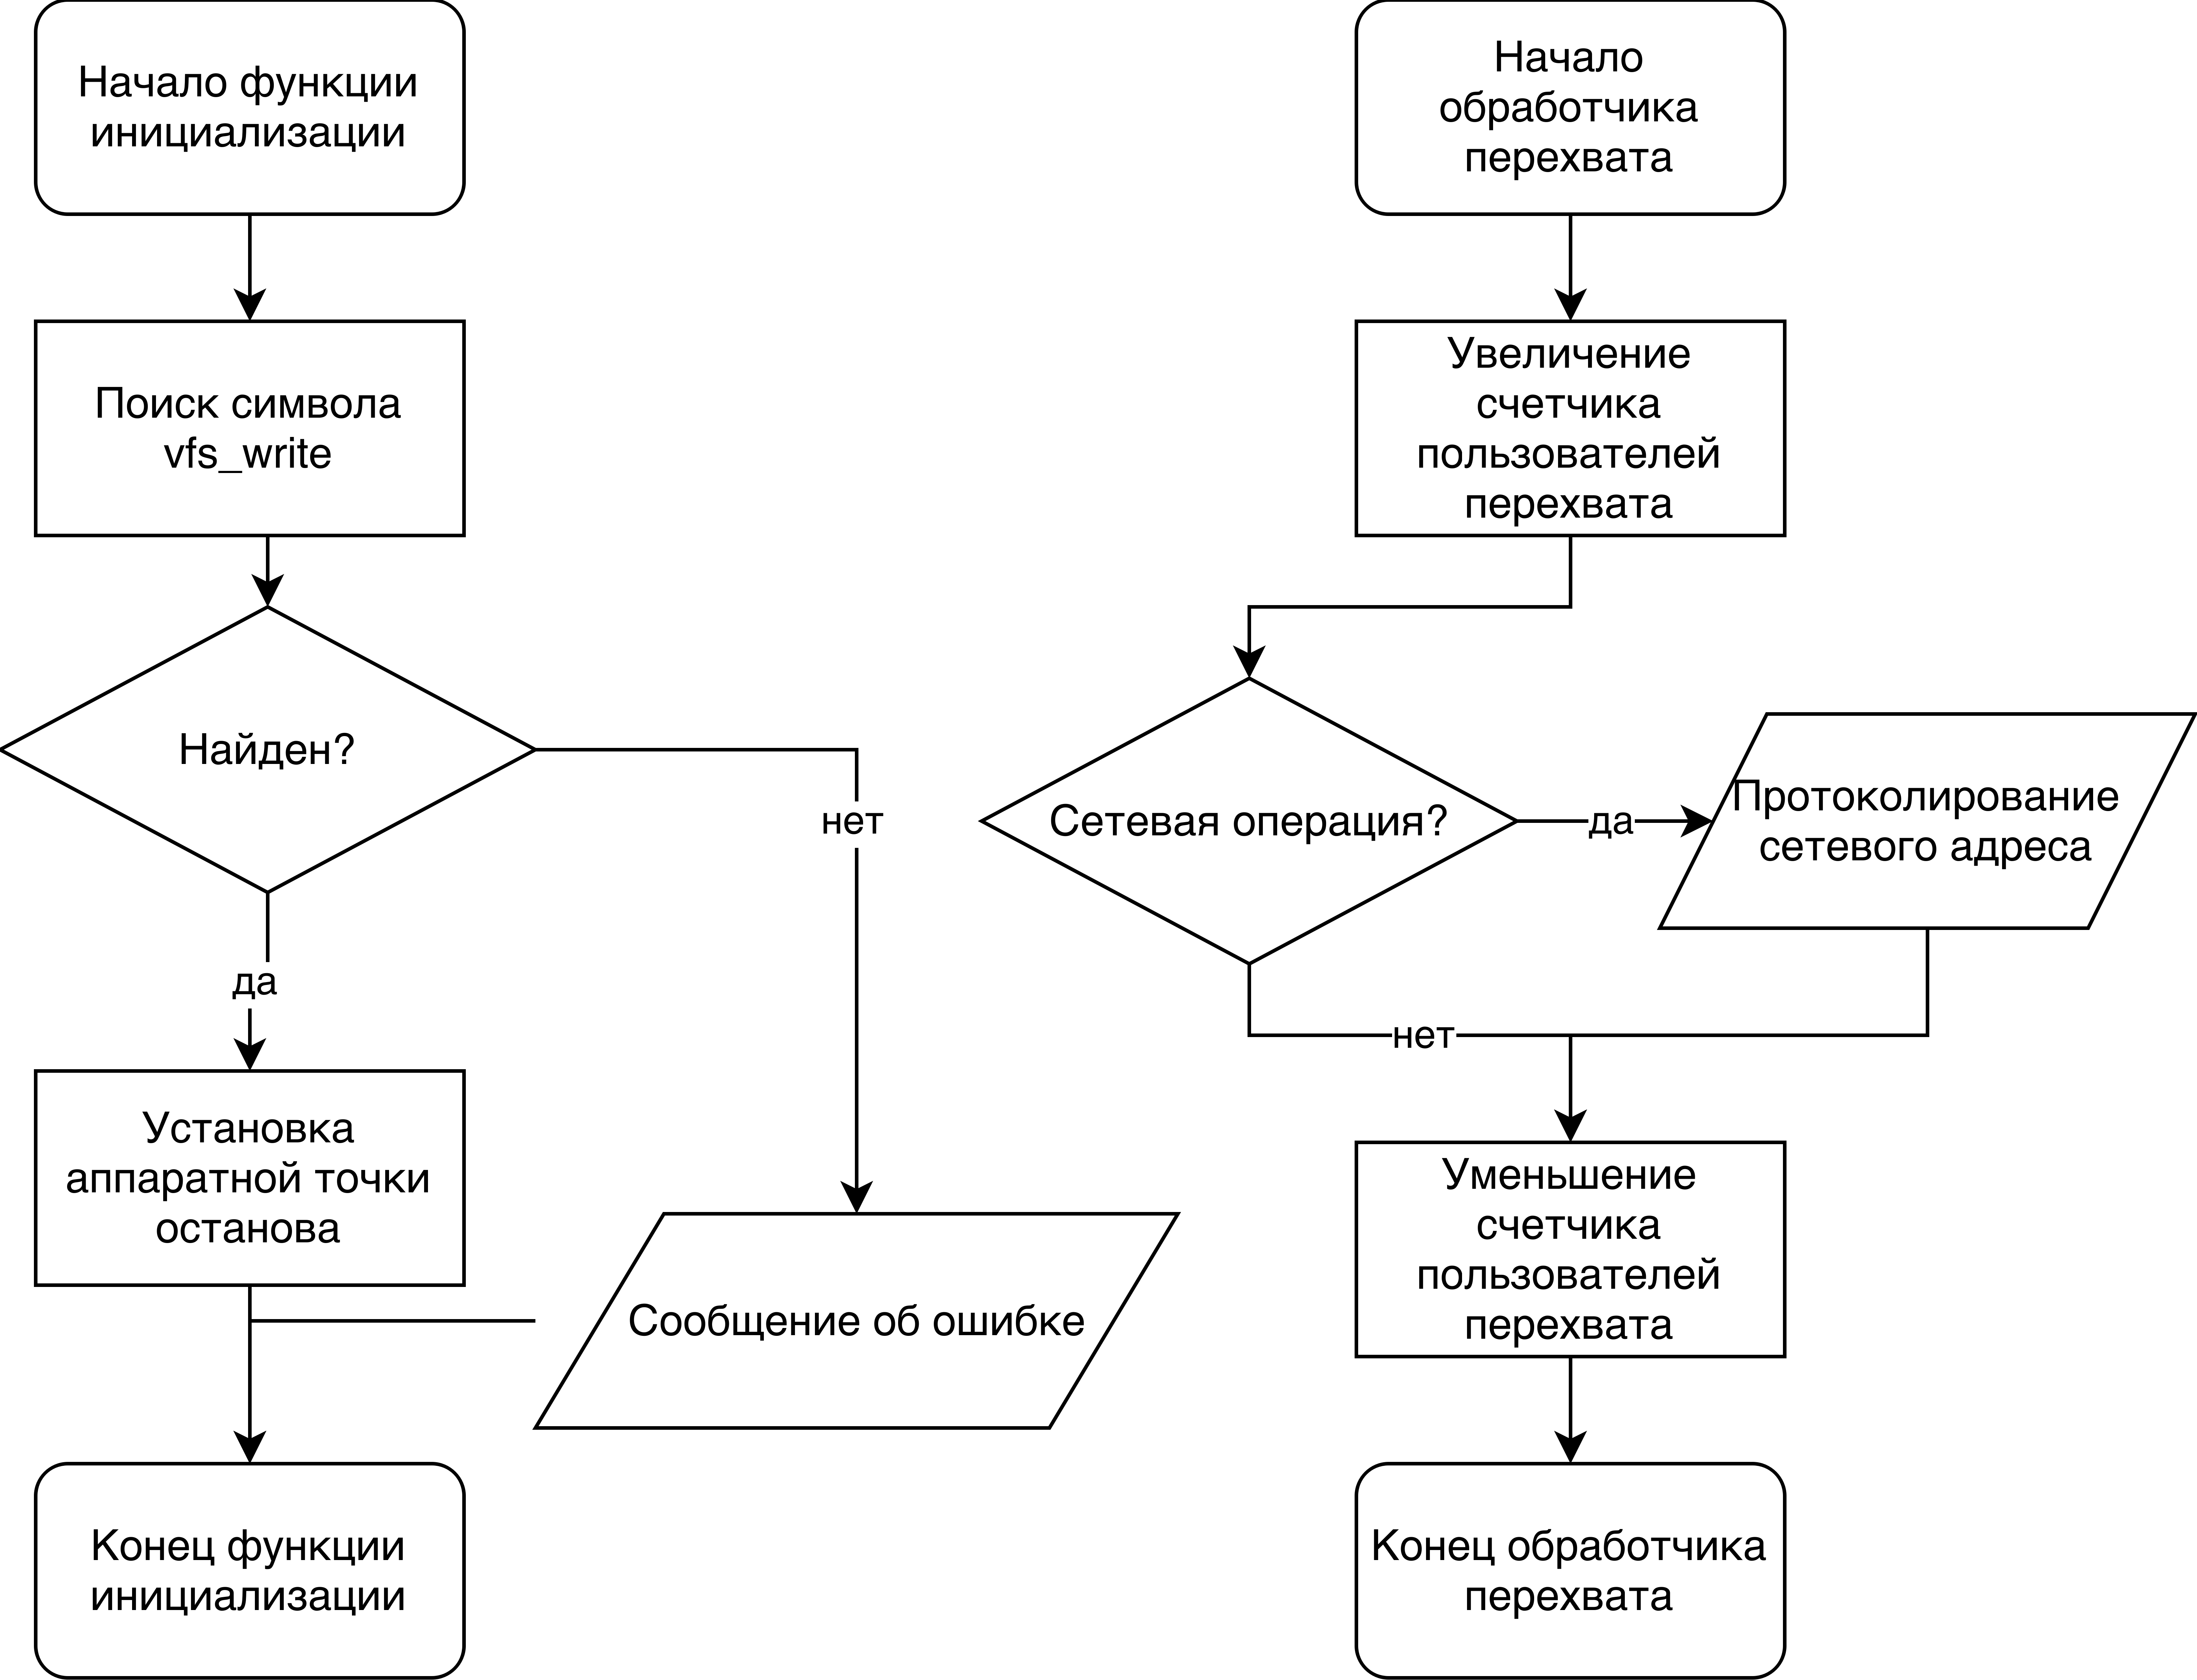
\includegraphics[width=0.9\textwidth]{images_posters/hook_net.png}
\vfill

\newpage
\hfill
\\
\vspace{2em}
Алгоритм функционирования метода выявления скрытых
объектов файловой системы
\vfill
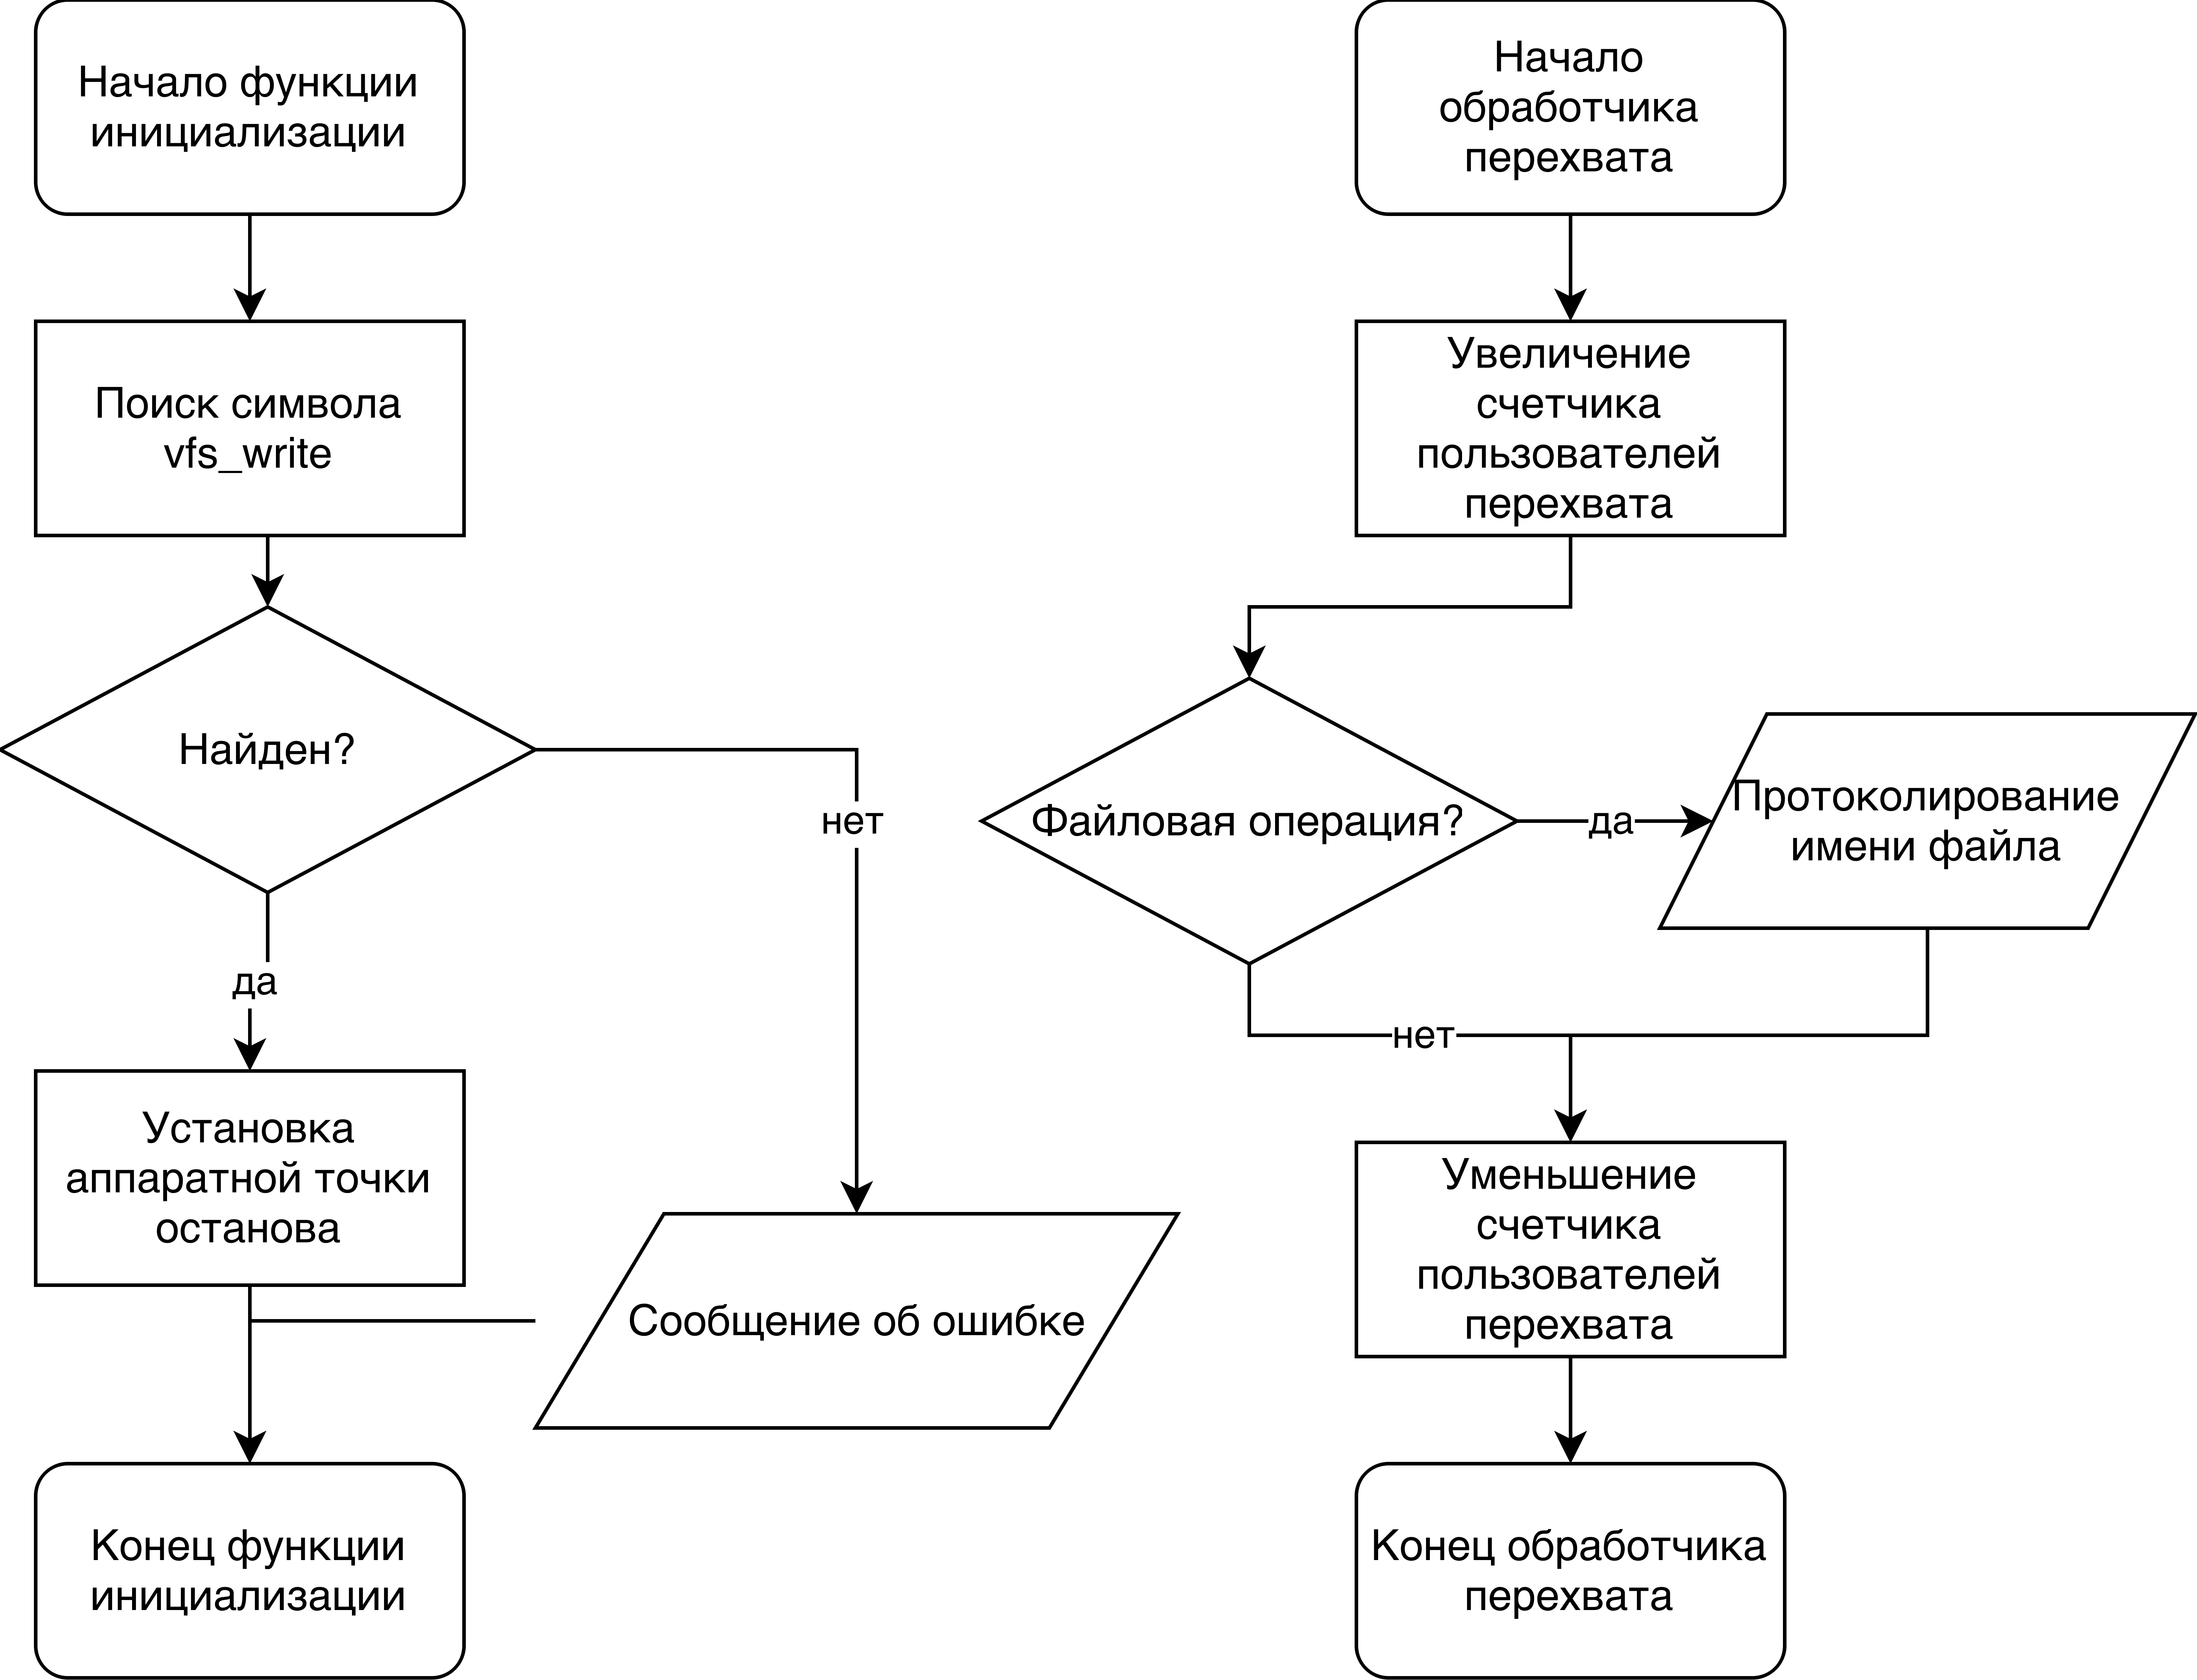
\includegraphics[width=0.9\textwidth]{images_posters/hook_fs.png}
\vfill

\newpage
\hfill
\\
\vspace{2em}
Схема планировщика задач ядра Linux
\vfill
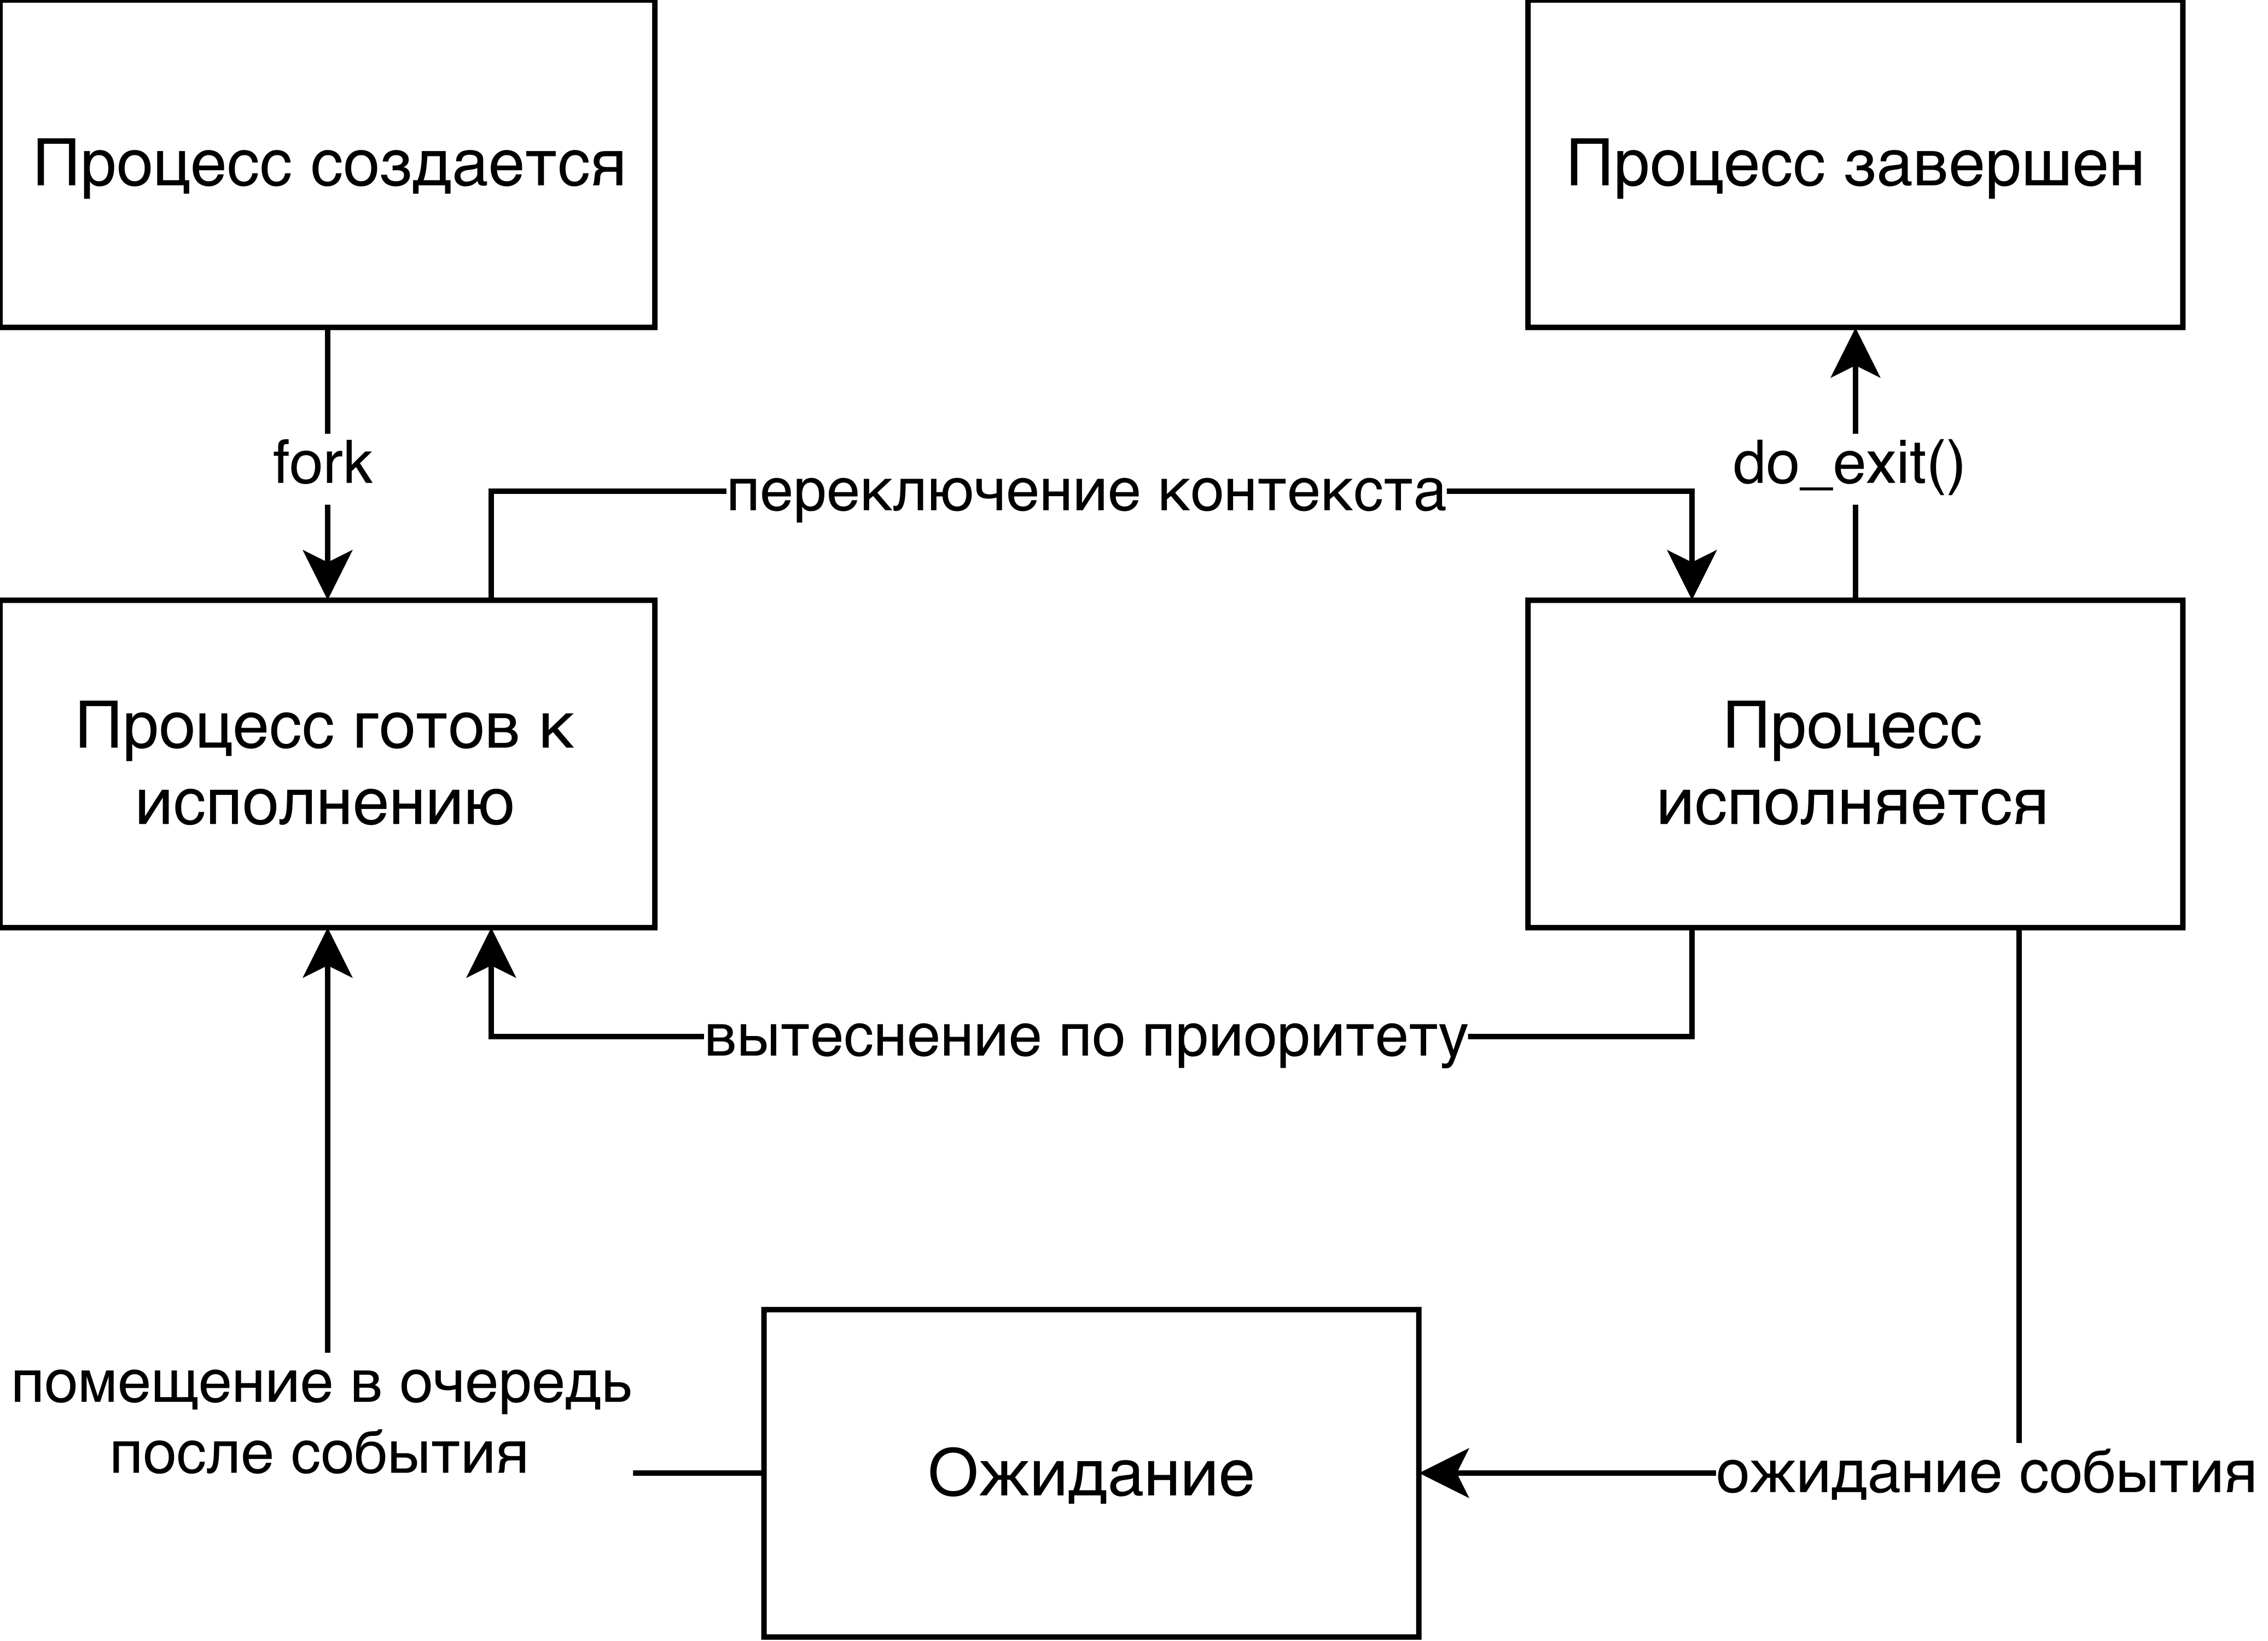
\includegraphics[width=0.9\textwidth]{images_posters/scheduler.png}
\vfill

\newpage
\hfill
\\
\vspace{2em}
Схема слоя виртуальных файловых систем ядра Linux
\vfill
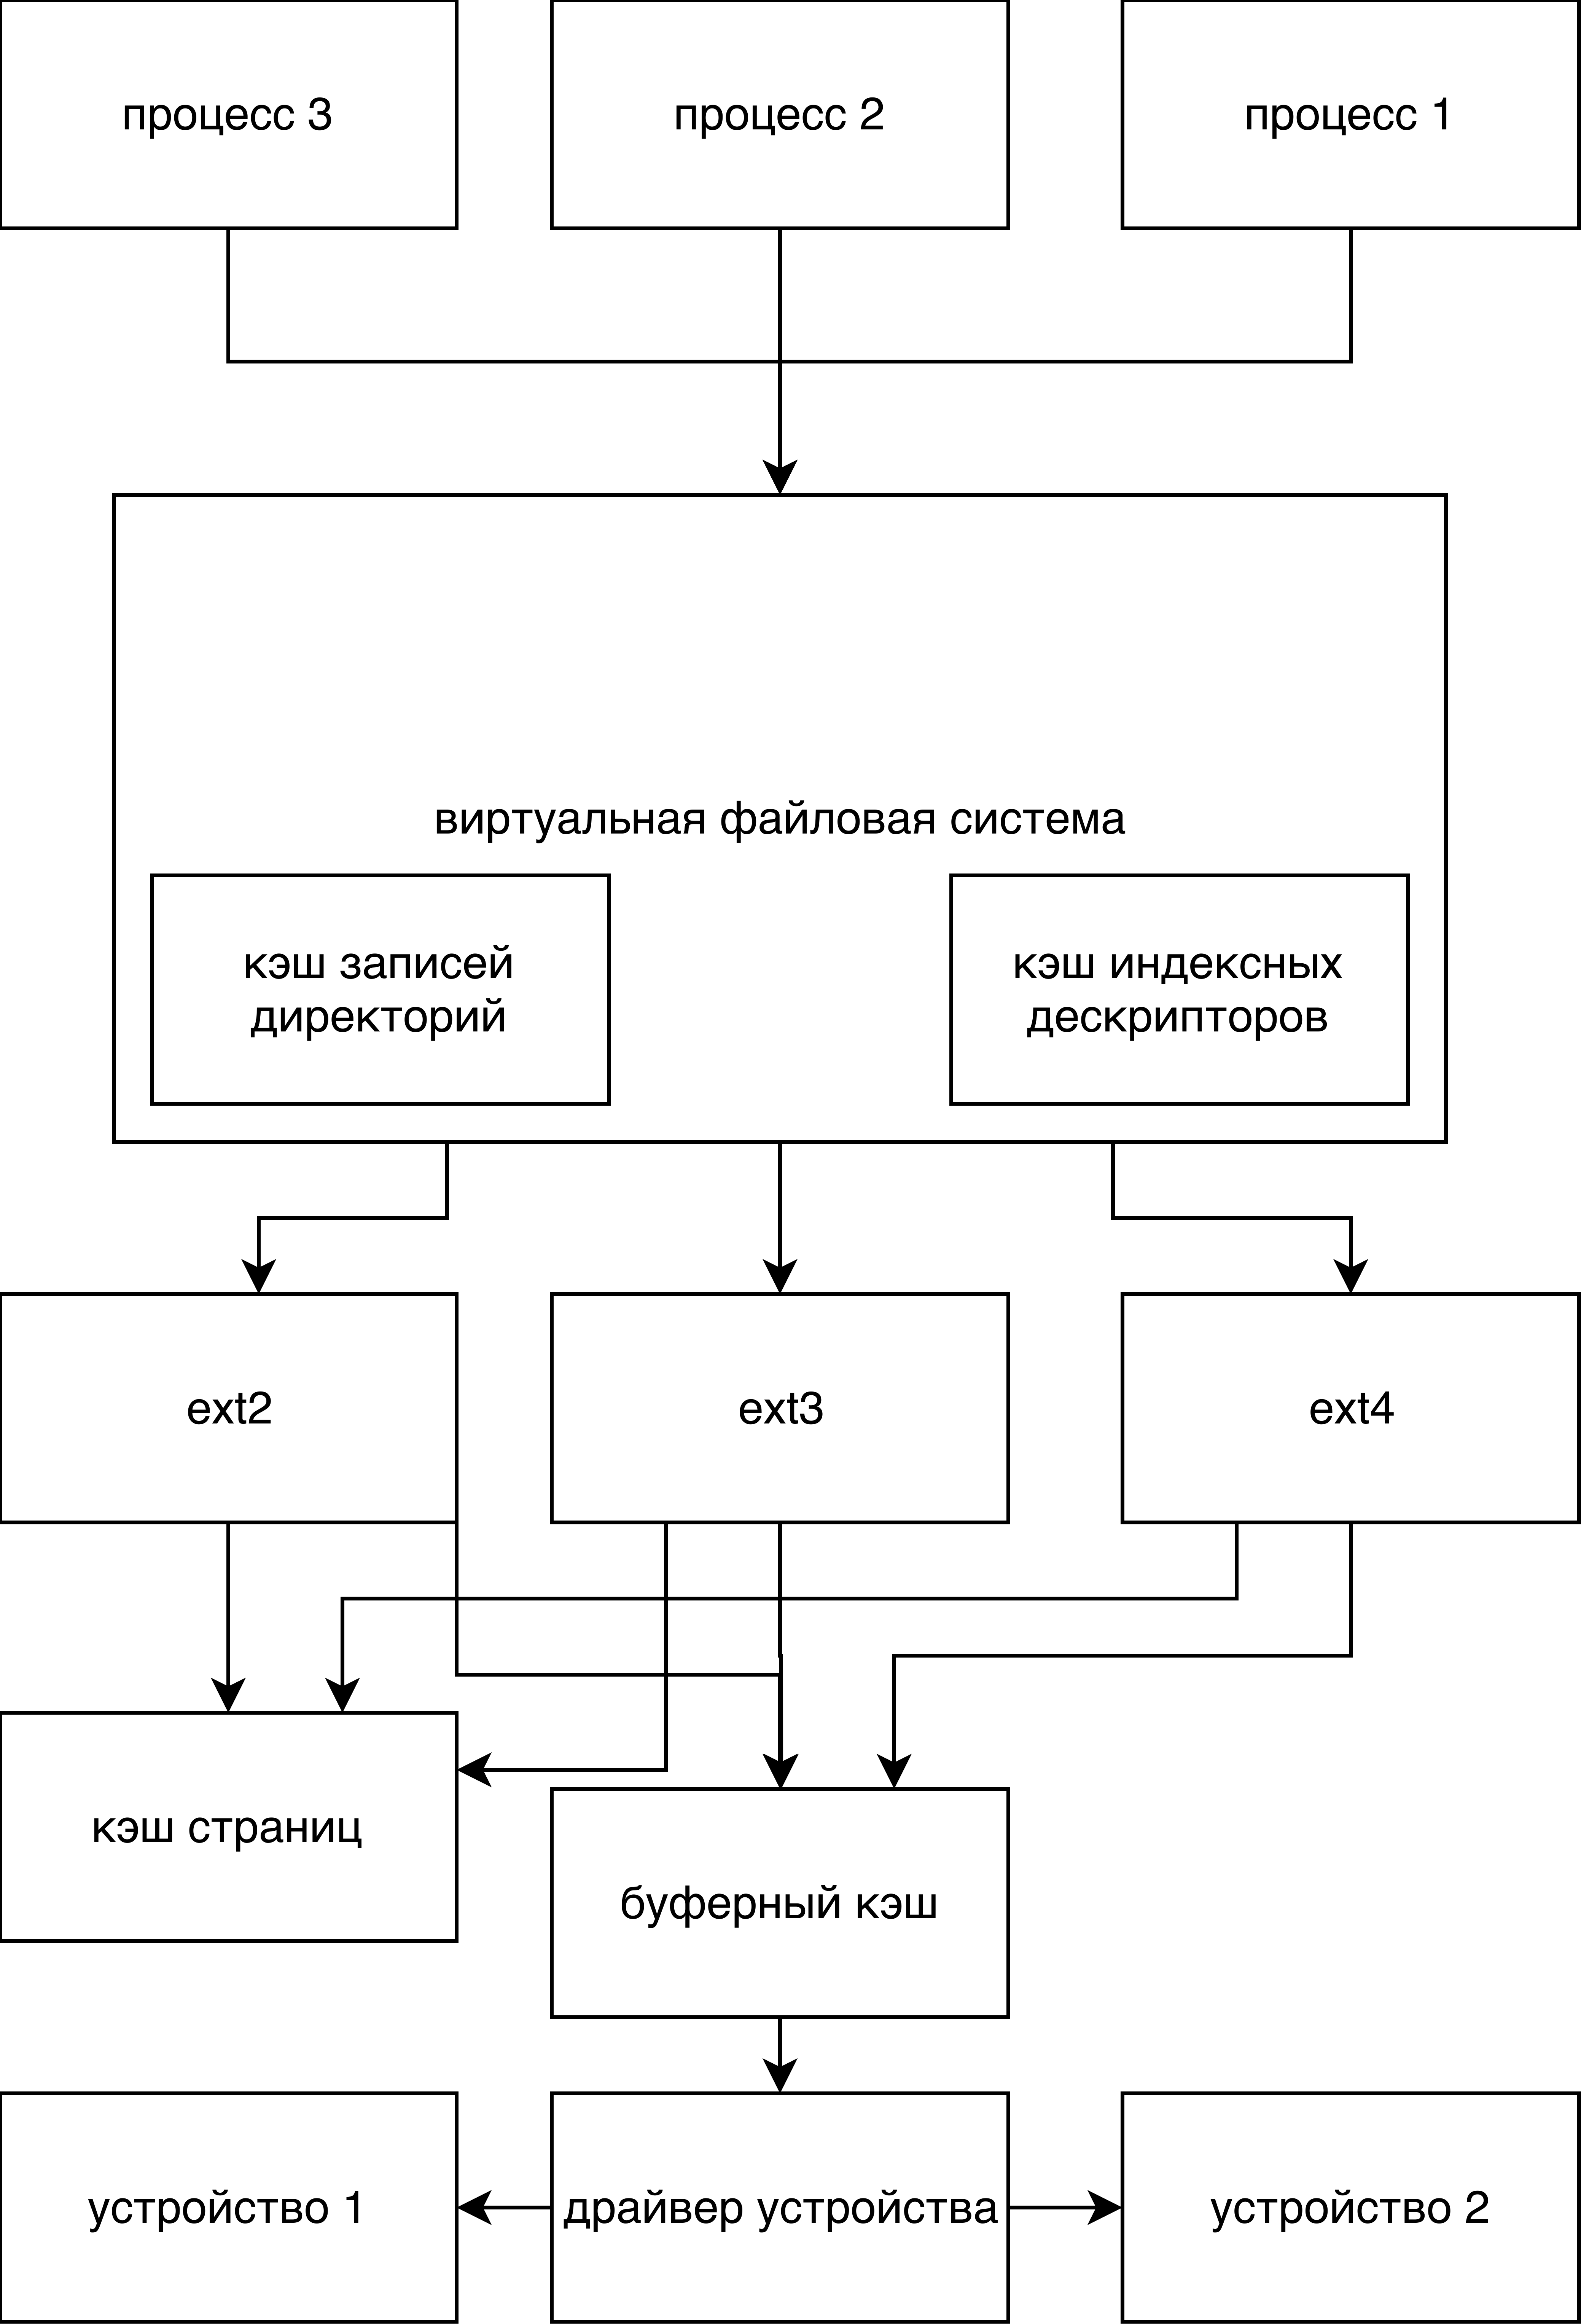
\includegraphics[width=0.8\textwidth]{images_posters/vfsscheme.png}
\vfill

\newpage
\hfill
\\
\vspace{2em}
Схема сетевого стека ядра Linux
\vfill
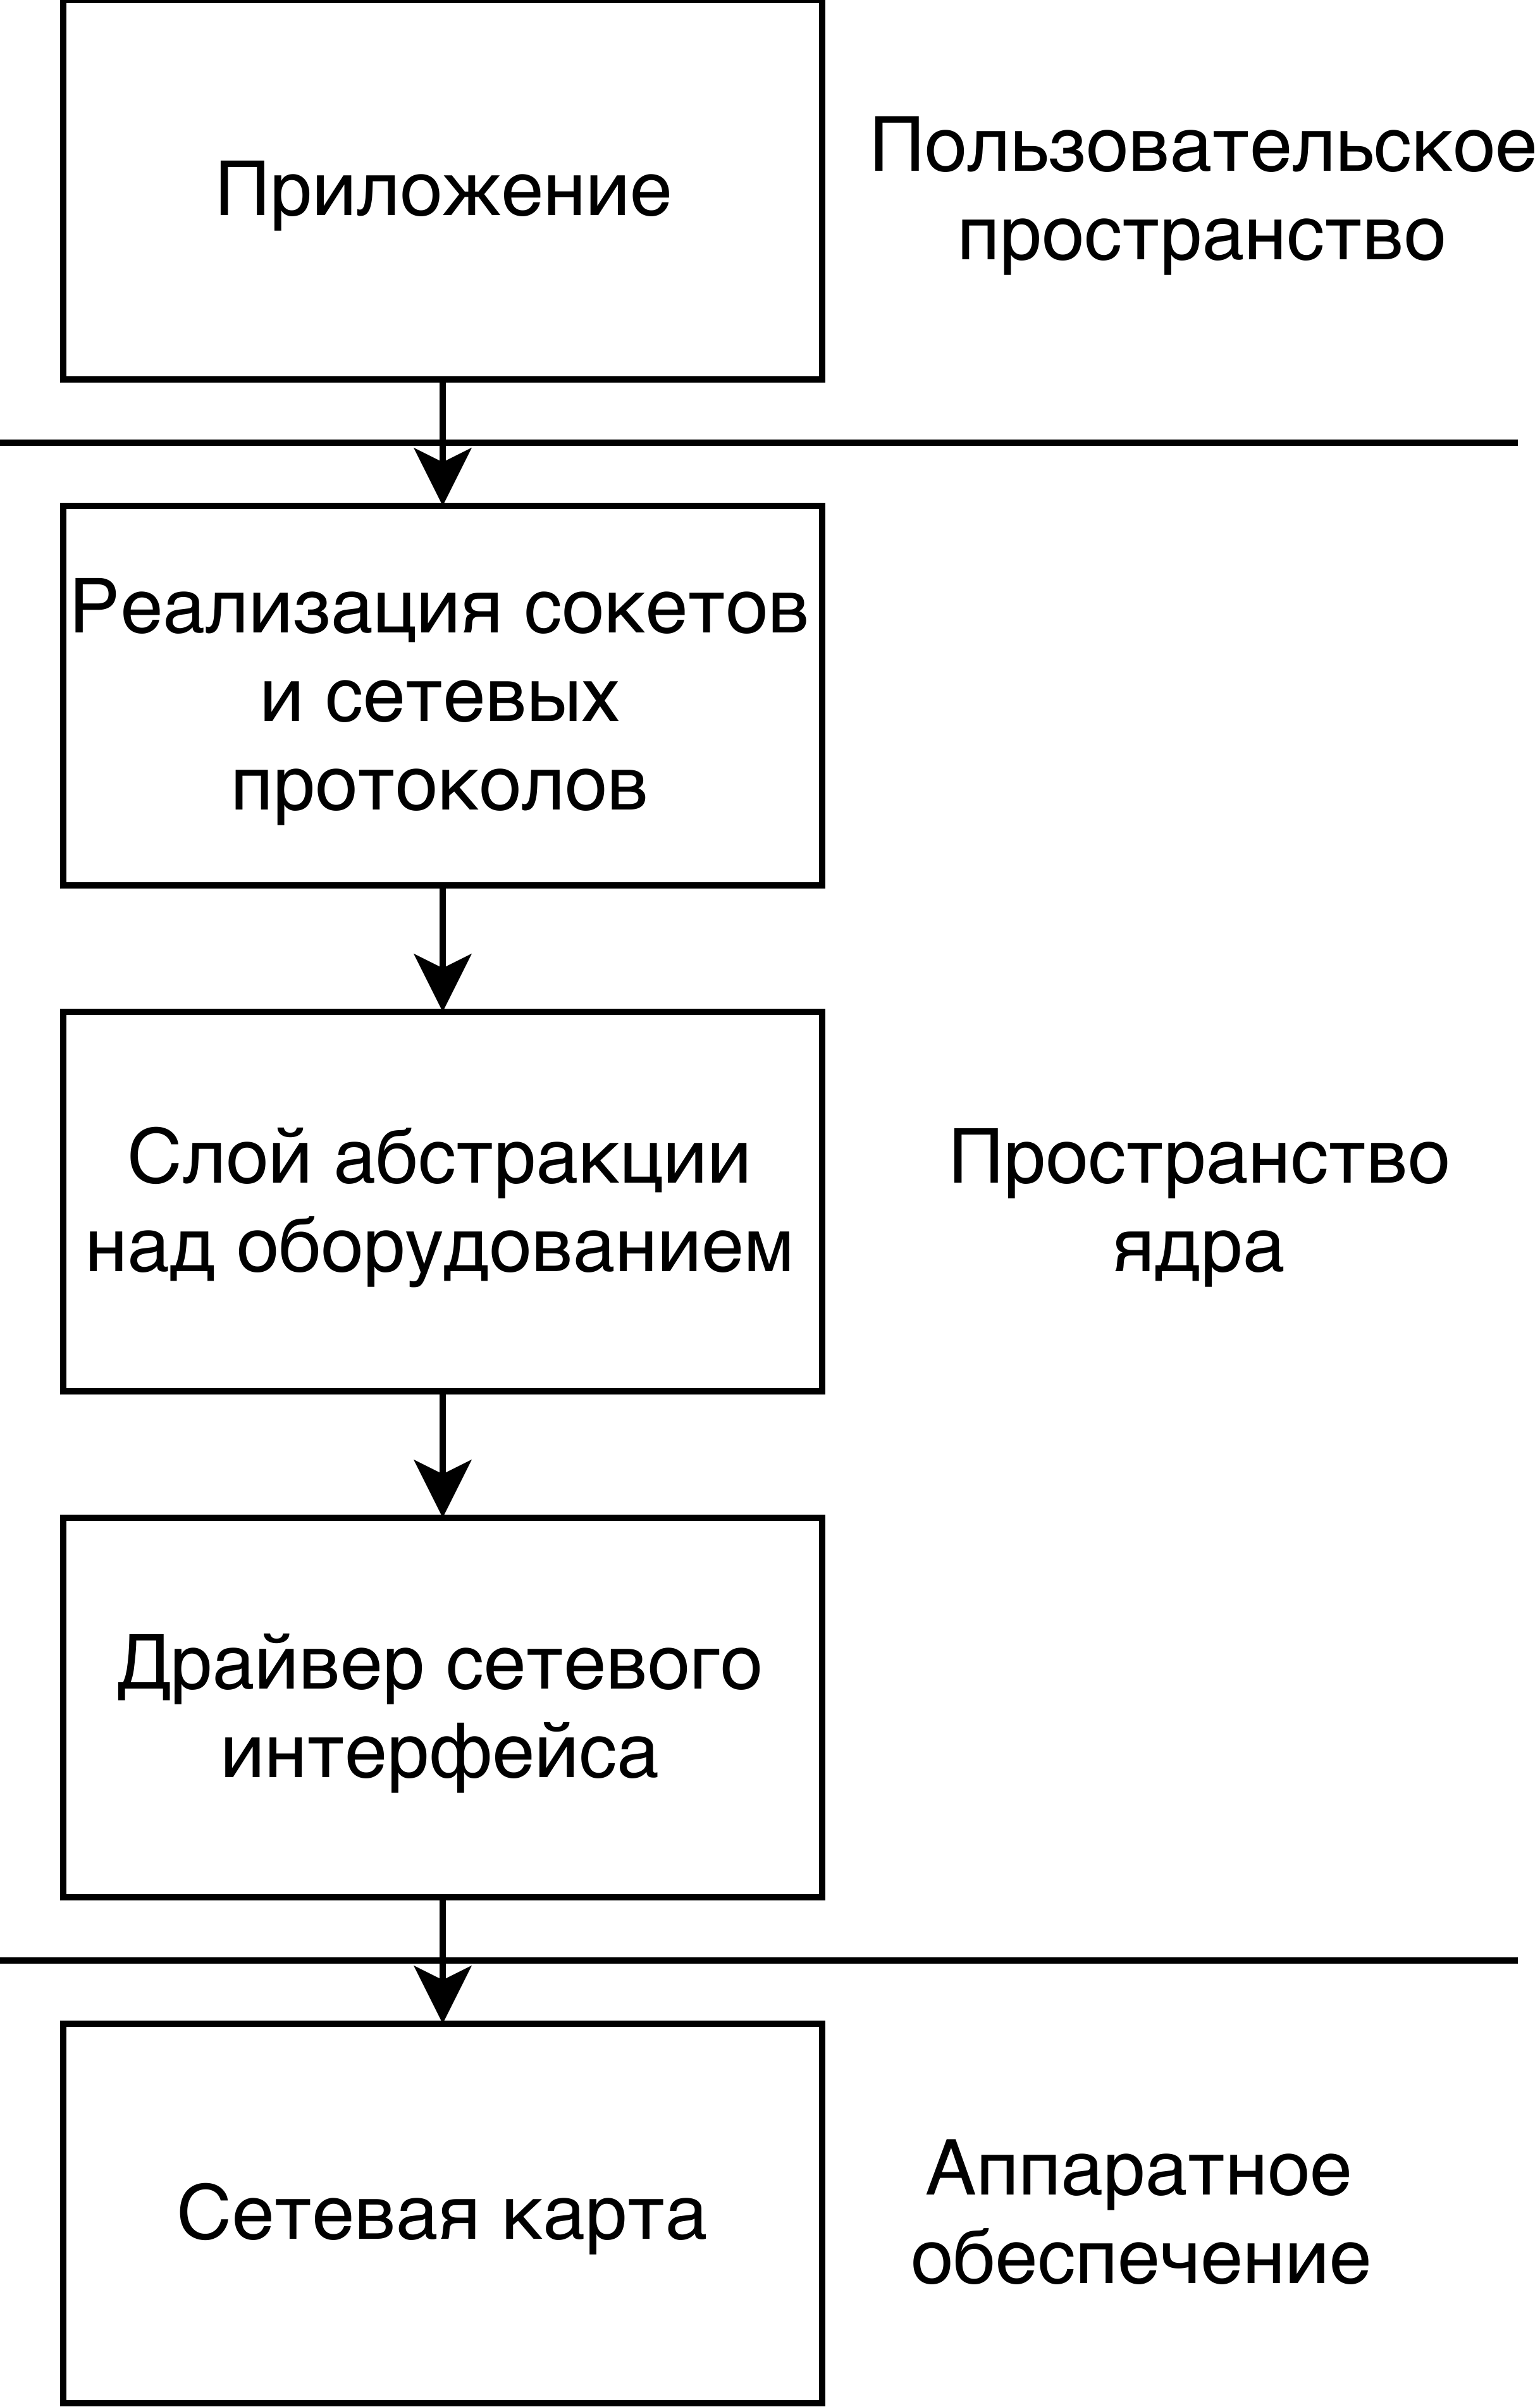
\includegraphics[width=0.6\textwidth]{images_posters/networking.png}
\vfill

\end{document}
